% Full instructions available at:
% https://github.com/elauksap/focus-beamertheme

\documentclass{beamer}
\usetheme[numbering=progressbar]{focus}
\usepackage{tikz}
\usetikzlibrary{positioning}
\usetikzlibrary{shapes,arrows}
\usepackage{transparent}
\usepackage{fancyvrb}
\usepackage{listings}
\usepackage{csquotes}
\definecolor{main}{RGB}{47, 161, 219}
%\definecolor{textcolor}{RGB}{128, 128, 128}
\definecolor{background}{RGB}{240, 247, 255}
\definecolor{textcolor}{RGB}{85, 87, 83}
\title{D4 Project}
\subtitle{Revamping Passive SSL with D4}
\author{Jean-Louis Huynen}
\titlegraphic{
\includegraphics[width=140pt]{d4-logo.pdf}}
\institute{Team CIRCL \\ \url{https://www.d4-project.org/}}
\date{20190329}
 \lstset{%
        language=bash,
        backgroundcolor=\color{gray!25},
        basicstyle=\ttfamily,
        breaklines=true,
        columns=fullflexible
    }
\begin{document}

\begin{frame}
    \maketitle
\end{frame}
       
\begin{frame}
        \frametitle{A passive SSL fingerprinter}
        CSIRT's rationale for collecting TLS handshakes:
        \begin{itemize}
          \item pivot on additional data points,
          \item find owners of IP addresses,
          \item detect usage of CIDR blocks,
          \item detect vulnerable systems,
          \item detect compromised services,
          \item detect Key material reuse.
        \end{itemize}
\end{frame}

\begin{frame}
  \frametitle{Objectives}

        History of links between:
        \begin{itemize}
          \item x509 certificates (And therefore their fields),
          \item ports,
          \item IP address,
          \item client (ja3),
          \item server (ja3s),
        \end{itemize}
        \begin{displayquote}
        ``JA3 is a method for creating SSL/TLS client fingerprints that should be easy to produce on any platform and can be easily shared for threat intelligence.''\footnote{https://github.com/salesforce/ja3}
        \end{displayquote}
\end{frame}
 
\begin{frame}
        \frametitle{Problem statement}
        \begin{itemize}
          \item CIRCL already offers a similar service based on SSLDump\footnote{https://www.circl.lu/services/passive-ssl/},
          \item SSLDump needs some love - maintaining it is hard,
          \item SSLDump needs some love - extending it even harder,
          \item nlternatives do not span the entire TLS Handshake (Salesforce's
            ja3\footnote{https://github.com/salesforce/ja3}),
          \item TCP reassembly is not an easy problem to solve (Cloudfare's uses tshark\footnote{https://github.com/cloudflare/mitmengine}),
        \end{itemize}
\end{frame}

\begin{frame}
        \frametitle{sensor-d4-tls-fingerprinting}
        Main features:
        \begin{itemize}
          \item take over SSLDump's duty,
          \item written in Golang 
          \item uses Go packet for tcp reassembly and spans whole TLS handshake
          \item ja3, ja3s, certificates, ip src / dst, port src / dst, TLSH
        \end{itemize}
        Current caveats:
        \begin{itemize}
          \item Support for TLS 1.3 pending
          \item Reassembly consumes a lot of RAM
        \end{itemize}
\end{frame}

\begin{frame}
        \frametitle{sensor-d4-tls-fingerprinting}
        \begin{columns}
            \begin{column}{0.5\textwidth}
              \begin{center}
                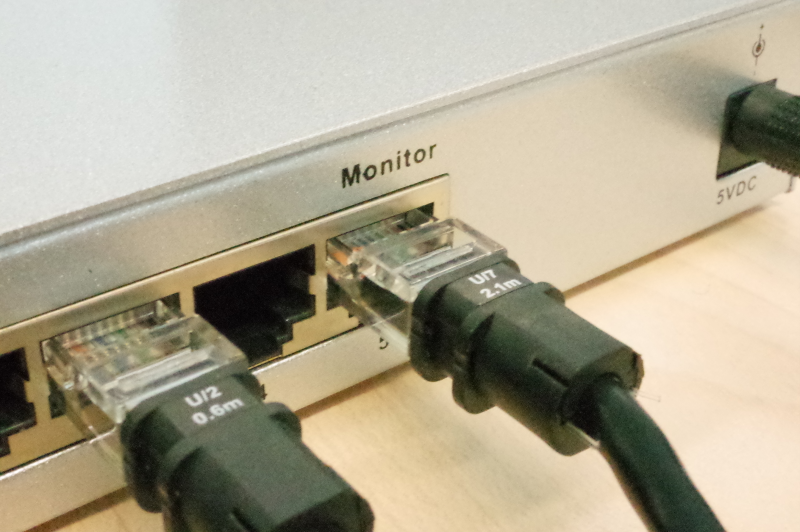
\includegraphics[scale=0.2]{../../informal-preso/0-intro-banana/monitor.png}
              \end{center}
            \end{column}
            \begin{column}{0.5\textwidth} 
              \begin{center}
                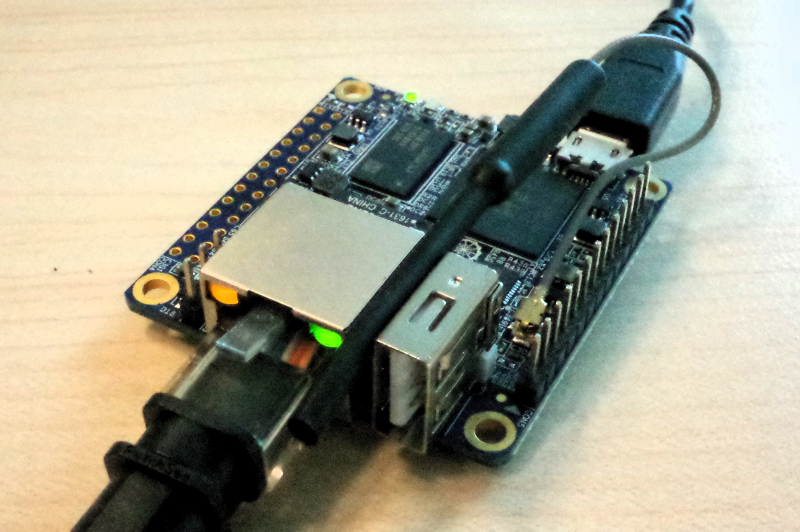
\includegraphics[scale=0.2]{../../informal-preso/0-intro-banana/orangepi.png}
              \end{center}
            \end{column}
          \end{columns}
          \hspace{20pt}
          \begin{itemize}
            \item 1 desktop monitored during 15 days
            \item 3327 TLS sessions fingerprinted
            \item 600 unique certificates collected
          \end{itemize}
\end{frame}

\begin{frame}
        \frametitle{sensor-d4-tls-fingerprinting - collection}

  \begin{lstlisting}
./d4-tlsf-amd64 -r|-i [-w -j -d -mbpc -mbpt -v] 
\end{lstlisting}



\begin{tabular}{l|l}
Options & Explanations\\
\hline
  -r & read pcap file\\
  -i & read from the interface \\
  -w & dump certificates to folder\\
  -j & write TLS session JSON descriptions to folder\\
  -mbcp & max buffered pages per connection (16) \\
  -mbpt & max total buffered pages (1024) \\
  -d & debug \\
  -v & verbose
\end{tabular}

\vspace{.8cm}
Available on the D4 project's github page\footnote{\url{github.com/D4-project/sensor-d4-tls-fingerprinting}}.
Depends on libpcap.

\end{frame}


\begin{frame}[fragile]
        \frametitle{sensor-d4-tls-fingerprinting | d4 client} 
        Required setting:
        \begin{itemize}
        \item type should be set to 2 or 254
          \item metaheader.json should state type: ja3-jl
        \end{itemize}
        \input{metaheader.json}
        \vspace{.5cm}
        \begin{lstlisting}
./d4-tlsf-amd64 -i eth0 | ./d4-amd64 -c conf.crq
\end{lstlisting}
        In the present setting the sensor will:
        \begin{itemize}
          \item describe every TLS Sessions,
          \item marshal this description in JSON format
          \item ship this description to D4 server
        \end{itemize}
\end{frame}

\begin{frame}
        \frametitle{sensor-d4-tls-fingerprinting - ja3-jl plugin} 
              \begin{center}
                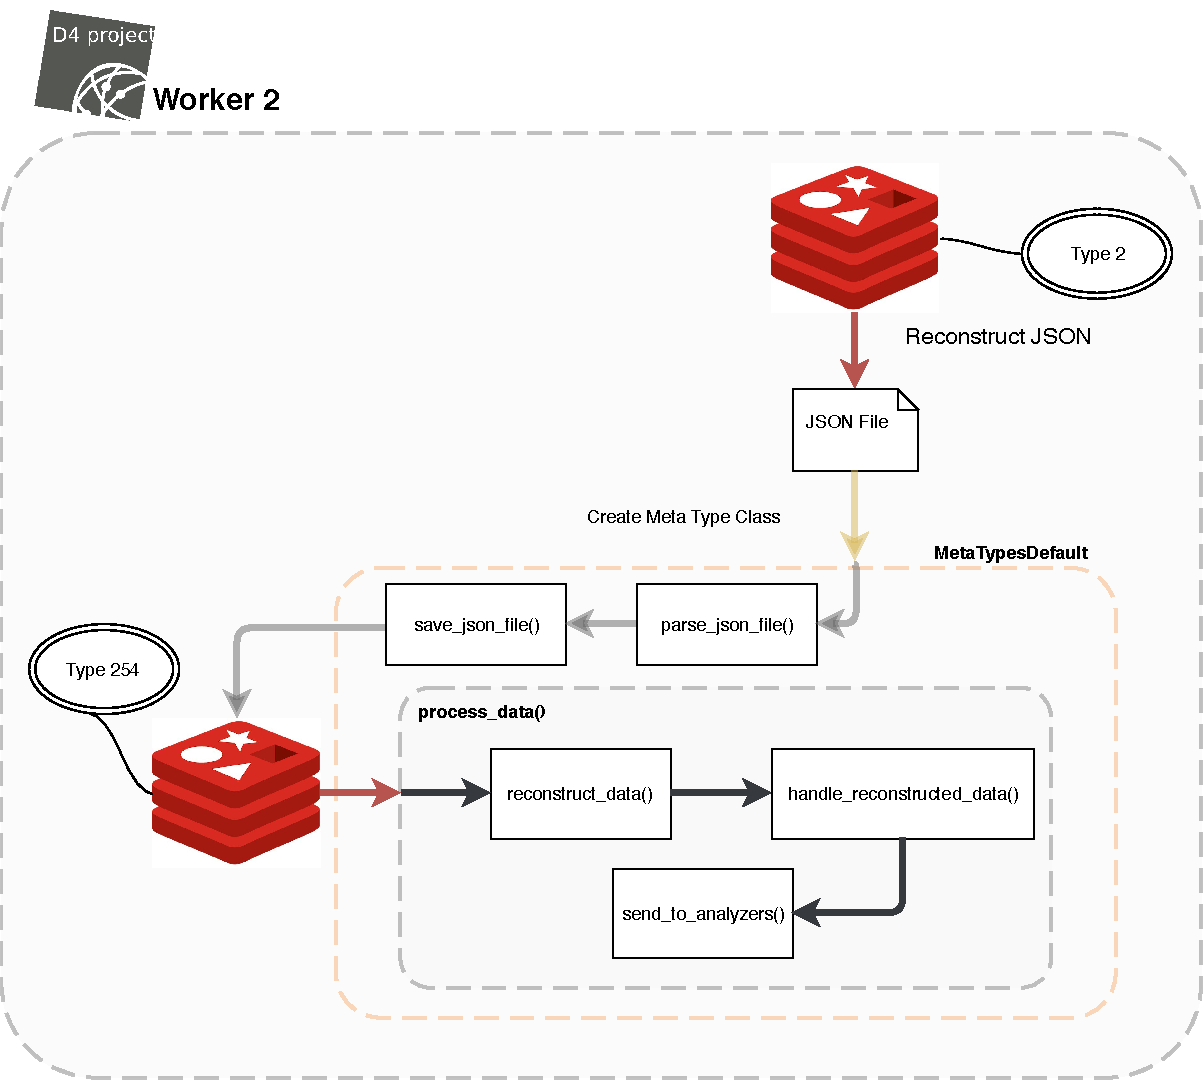
\includegraphics[scale=0.4]{d4-worker2-ja3-jl.pdf}
              \end{center}
\end{frame}

\begin{frame}[fragile]
        \frametitle{sensor-d4-tls-fingerprinting - ja3-jl worker} 
        \begin{lstlisting}
    def __init__(self, uuid, json_file):
        super().__init__(uuid, json_file)
        self.set_rotate_file_mode(False)

    def process_data(self, data):
        self.reconstruct_data(data)

    def handle_reconstructed_data(self, data):
        ...
\end{lstlisting}
        \begin{itemize}
          \item processes each reassembled JSON description,
          \item extracts x509 certificates and write to disk,
          \item writes JSON description to disk,
          \item push the files paths to the analyzer.
        \end{itemize}
\end{frame}

\begin{frame}[fragile]
        \frametitle{sensor-d4-tls-fingerprinting - ja3-jl analyzer} 
        (Proof of Concept) \\
        \vspace{.8cm} 
        Populates a database:
        \begin{itemize}
          \item LPOP a redis list populated by the worker
          \item push JSON descriptions into a postgres database
        \end{itemize}
\end{frame}


\begin{frame}[fragile]
        \frametitle{sensor-d4-tls-fingerprinting - passivessl API} 
        (Proof of Concept) \\
        \vspace{.8cm} 
        Exposes a REST API to query the collected data:
        \begin{itemize}
          \item /index : returns the full DB (PoC), 
          \item /ja3/ : returns all TLS sessions with a given JA3 Signature,
          \item /ja3s/ : returns all TLS sessions with a given JA3S Signature,
        \end{itemize}
\end{frame}


\begin{frame}
\frametitle{Get in touch if you want to join the project, host a sensor or contribute}
\begin{itemize}
\item Collaboration can include research partnership, sharing of collected streams or improving the software.
\item Contact: info@circl.lu
\item \url{https://github.com/D4-Project} -  \url{https://twitter.com/d4_project}
\end{itemize}
\end{frame}


\end{document}
